\textbf{{1. TCP报文的首部格式}}

\textbf{{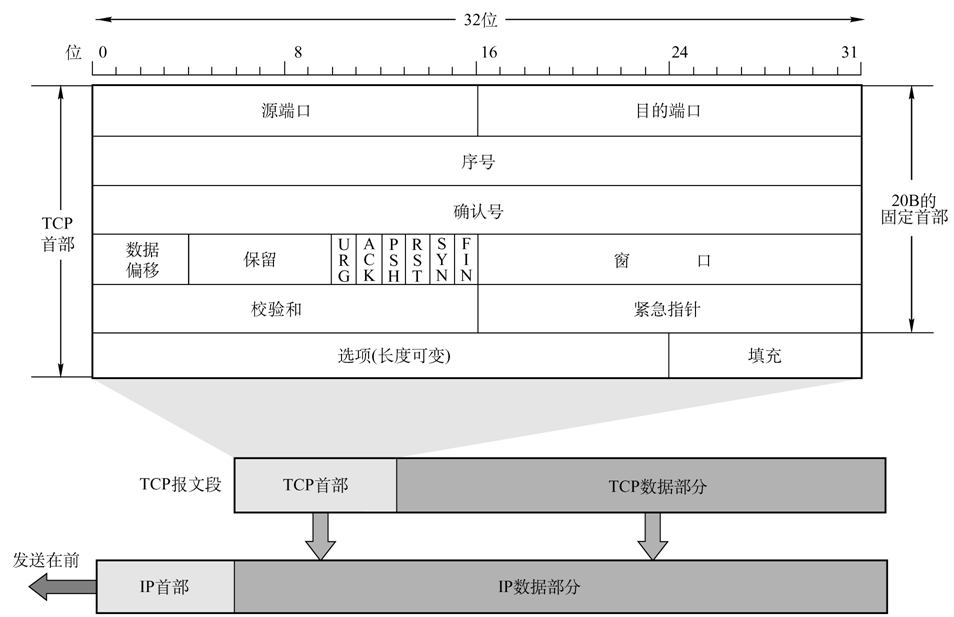
\includegraphics[width=3.54167in,height=2.29167in]{png-jpeg-pics/75C7D85D81D38FABFB6DC1B40CC50A32.png}\\
}}

\textbf{1)源端口和目的端口。}{各占2B。}

\textbf{2)序号。}占4B。尽管从应用层交付下来的是TCP报文段,但是TCP是面向字节流的(就是说TCP传送时是按照一个个字节来传送的),所以在一个TCP连接中传送的字节流需要编号,这样才能保证按序交付。

\textbf{3)确认号。}占4B。TCP是含有确认机制的,所以接收端需要给发送端发送确认号。

\textbf{4)数据偏移。}占4位。占4位可表示0001~1111一共15种状态,而基本单位是4B,所以数据偏移确定了首部最长为60B。

\textbf{5)保留字段。}占6位。保留为今后使用。

\textbf{6)紧急URG。}当URG=1时,表明紧急指针字段有效。它告诉系统此报文段中有紧急数据,应尽快传送(相当于高优先级的数据)。

\textbf{7)确认比特ACK。}只有当ACK1时确认号字段才有效。当ACK0时,确认号无效。TCP规定,一旦连接建立了,所有传送的报文段都必须把ACK置1。

\textbf{8)推送比特PSH。}TCP收到推送比特置1的报文段,就尽快地交付给接收应用进程,而不再等到整个缓存都填满后再向上交付。

\textbf{9)复位比特RST。}当RST1时,表明TCP连接中出现严重差错(如由于主机崩溃或其他原因),必须释放连接,然后再重新建立传输连接。

\textbf{10)同步比特SYN。}同步比特SYN置为1,表示这是一个连接请求或连接接受报文,后面TCP连接会详细讲到。

\textbf{11)终止比特FIN。}释放一个连接。当FIN1时,表明此报文段的发送端的数据已发送完毕,并要求释放传输连接。

\textbf{12)窗口字段。}占2B。窗口字段用来控制对方发送的数据量,单位为字节(B)。记住一句话:窗口字段明确指出了现在允许对方发送的数据量。

\textbf{13)校验和字段。}占2B。校验和字段检验的范围包括首部和数据两部分。在计算校验和时,和UDP一样,要在TCP报文段的前面加上12B的伪首部(只需将UDP伪首部的第4个字段的17改为6,其他和UDP一样)。

\textbf{14)紧急指针字段。}占2B。前面已经讲过紧急指针指出在本报文段中的紧急数据的最后一个字节的序号。

\textbf{15)选项字段。}长度可变。TCP最初只规定了一种选项,即最大报文段长度MSS。MSS告诉对方TCP:``我的缓存所能接收的报文段的数据字段的最大长度是MSS字节。''

\textbf{16)填充字段。}为了使整个首部长度是4B的整数倍。
